\documentclass{beamer}

\usepackage[ngerman]{babel}
\usepackage[utf8]{inputenc}
\usepackage[T1]{fontenc}
\usepackage{graphicx}

\usecolortheme{seagull}
\usefonttheme{serif}

\graphicspath{ {./images/} }

\title{Open-Source-Lizenzen}
\subtitle{Einordnung und Abgrenzung}
\author{Mara Schulke}

\AtBeginSection[]{
	\begin{frame}{Inhalt}
		\tableofcontents[currentsection]
	\end{frame}
}


\begin{document}

\maketitle

\section{Wieso sind Lizenzen so wichtig?}
\begin{frame}{Wieso sind Lizenzen so wichtig?}
\end{frame}

\section{FOSS:\ Free and Open Source Software}
\begin{frame}{FOSS:\ Free and Open Source Software}
	\begin{itemize}
		\item Umfasst jegliche quelloffene Software
		\item Nutzer kann Quellcode lesen, ändern und selber redistributieren
		\item Stellt die Entwicklung hochwertiger Software über wirtschaftliche
			Interessen
		\item Unternehemen verwenden i.d.R. FOSS um propräitäre Produkte darauf
			aufzubauen
	\end{itemize}
\end{frame}

\section{Lizenztypen}
\begin{frame}{Lizenztypen}
	\begin{itemize}
		\item Permissive
		\item Copyleft
	\end{itemize}
\end{frame}

\subsection{Permissive Lizenzen}
\begin{frame}{Lizenztypen:\ Permissive Lizenzen}
	\begin{itemize}
		\item haben einen freien und erlaubenden Charakter
		\item lassen Redistributionen unter anderen Lizenzen zu
		\item bestehen oft primär aus einem Haftungsausschluss, ohne
			nennenswerte weitere Vorgaben
		\item stellen den technischen Fortschritt über politische Debatten
	\end{itemize}
\end{frame}

\begin{frame}{Lizenztypen:\ Beispiele für Permissive Lizenzen}
	\begin{itemize}
		\item BSD-2-Clause License
		\item BSD-3-Clause License
		\item MIT License
		\item Apache 2.0 License
	\end{itemize}
\end{frame}

\subsection{Copyleft Lizenzen}
\begin{frame}{Lizenztypen:\ Copyleft Lizenzen}
	\begin{itemize}
		\item bekannt für sog.\ virale Lizensierung,
			verbieten Redistributionen unter anderen Lizenzen
		\item haben i.d.R. einen eher extremen / politischen Charakter (bspw. GPLv3)
		\item spiegeln Ideologie der Free-Software-Foundation wieder
		\item gemieden von propräitärer Software
	\end{itemize}
\end{frame}

\begin{frame}{Lizenztypen:\ Beispiele für Copyleft Lizenzen}
	Schwaches Copyleft
	\vspace{0.5em}
	\begin{itemize}
		\item GNU Lesser General Public License
		\item Mozilla Public License
		\item Eclipse Public License
	\end{itemize}
	\vspace{1em}

	Starkes Copyleft
	\vspace{0.5em}
	\begin{itemize}
		\item GNU General Public License
		\item GNU Affero General Public License
	\end{itemize}
\end{frame}

\section{Einordnung von Lizenzen}
\begin{frame}{Einordnung von Lizenzen}
	// spektrum einfügen
\end{frame}

\section{Lizenzen im Detail}
\subsection{GNU General Public License v2}
\begin{frame}{GNU General Public License v2}
	\begin{itemize}
		\item Lizenz muss bei Redistribution mit ausgeliefert werden
		\item Alle signifikanten Änderungen müssen gekennzeichnet werden
		\item Redistribution muss unter der gleichen Lizenz erfolgen
		\item Sobald Binärdateien basierend auf einem Projekt unter GPLv2
			ausgeliefert werden muss der Quellcode verfügbar gemacht werden
	\end{itemize}
\end{frame}

\subsection{GNU General Public License v3}
\begin{frame}{GNU General Public License v3}
	Strenges Copyleft,
	\begin{itemize}
		% Beide verlangen unter sich selbst redistributiert zu werden
		\item Inkopatibel zur GPLv2
	\end{itemize}
\end{frame}

\subsection{Apache 2.0 License}
\begin{frame}{Apache 2.0 License}
\end{frame}

\subsection{Mozilla Public License}
\begin{frame}{Mozilla Public License}
\end{frame}

\subsection{MIT License}
\begin{frame}{MIT License}
\end{frame}

\subsection{BSD License}
\begin{frame}{BSD License}
\end{frame}

\section{Unlizensierte Software}
\begin{frame}{Unlizensierte Software}
\end{frame}

\section{Daten zur Lizenznutzung auf GitHub}
\begin{frame}{Daten zur Lizenznutzung auf GitHub: Verteilung}
	\begin{figure}[ht]
		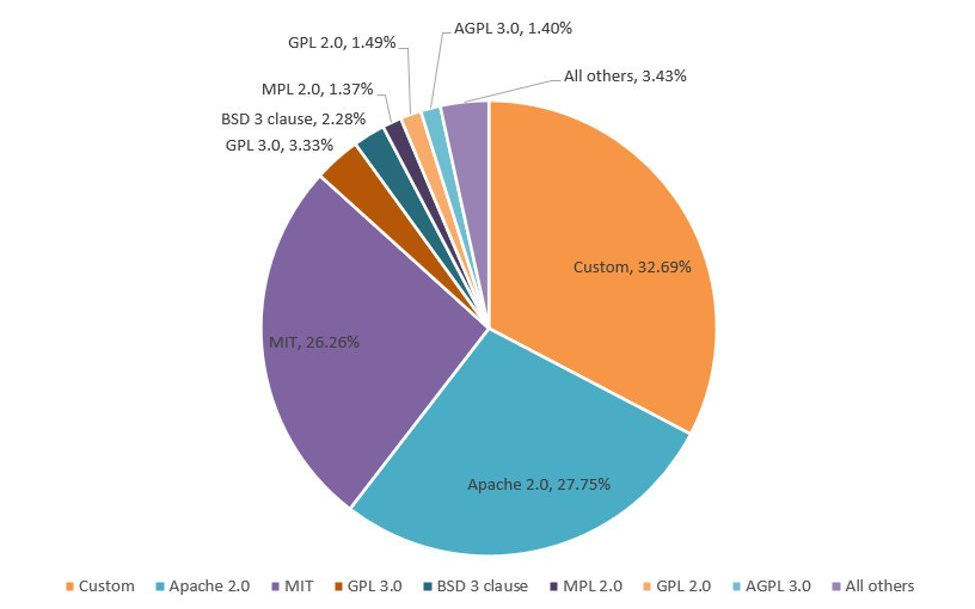
\includegraphics[width=0.75\textwidth]{lizenzverteilung}
		\centering
		\caption{Lizenzverteilung auf GitHub (2018-2020)}
		Quelle: Solutionshub 2020
	\end{figure}
\end{frame}

\begin{frame}{Daten zur Lizenznutzung auf GitHub: Trends}
	\begin{figure}[ht]
		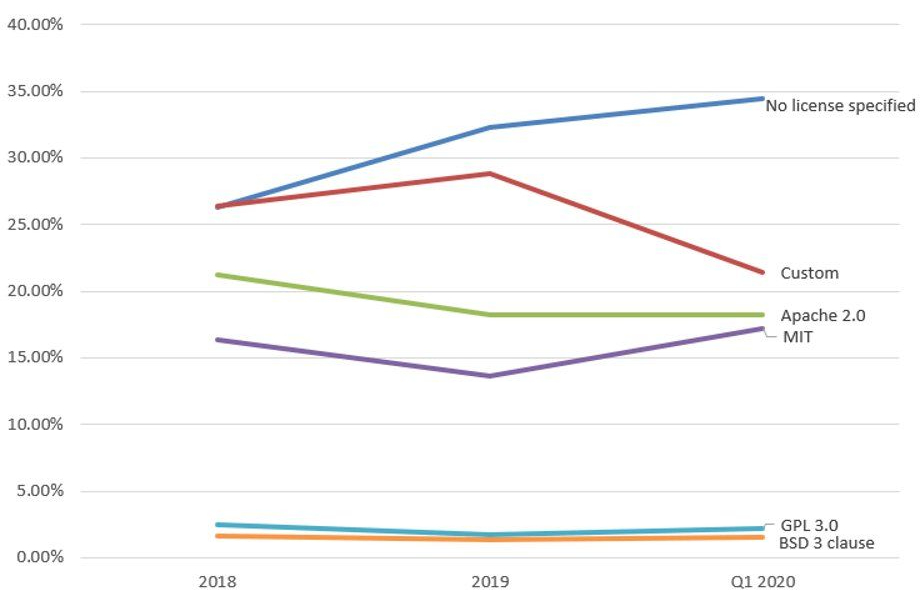
\includegraphics[width=0.75\textwidth]{trend}
		\centering
		\caption{Trends der Lizenznutzung (2018-2020)}
		Quelle: Solutionshub 2020
	\end{figure}
\end{frame}

\section{Rechtsfolgen von Lizenzverstößen}
\begin{frame}{Rechtsfolgen von Lizenzverstößen}
\end{frame}

\section{Fragen}
\begin{frame}{Fragen}
	\begin{itemize}
		\item Welche Faktoren müssen bei der Lizenzwahl beachtet werden?
			% Finde ich es okay wenn jemand mit meiner Arbeit Geld verdient?
			% Soll diese Arbeit immer Open Source bleiben?
			% Habe ich eine Marke die ich Schützen will?
		\item Wodurch zeichnet sich der Copyleft-Effekt aus? % Virale Lizensierung
	\end{itemize}
\end{frame}

\section{Quellen}
\begin{frame}{Quellen}
% https://solutionshub.epam.com/blog/post/examining-open-source-license-usage



% https://choosealicense.com/licenses/
% https://www.gnu.org/licenses/license-list.de.html#GPLCompatibleLicenses
% https://www.gnu.org/licenses/copyleft
% https://www.ifross.org/?q=urteile
\end{frame}

%# Definition Open Source

%# Gesetzes Grundlage für Lizenzen bzw. Nutzungsrechte

%https://www.gesetze-im-internet.de/urhg/__69d.html
%https://www.gesetze-im-internet.de/urhg/__16.html
%https://de.wikipedia.org/wiki/Lizenz

%> Für das bloße Ausführen eines Programms im nicht-öffentlichen Rahmen ist keine Lizenz erforderlich, da dies keinem Verbot unterliegt. Eine urheberrechtliche Lizenz, also eine urheberrechtliche Nutzungs-/Verwertungserlaubnis, ist bei urheberrechtlich geschützten Computerprogrammen nur erforderlich, wenn eine urheberrechtlich relevante Nutzungs-/Verwertungshandlung erfolgt, die nicht bereits durch die in § 69d Abs. 1 UrhG verankerte gesetzliche Lizenz erfasst ist. Vor allem aus dem Lager der großen Softwarehersteller wird dies regelmäßig negiert bzw. in Abrede gestellt und hierzu auch gerne versucht, bereits den Lauf eines Computerprogramms als urheberrechtliche Verwertungshandlung erscheinen zu lassen. Ignoriert wird hierbei aber, dass nicht jeder technische Kopiervorgang, wie er definitiv beim Lauf eines Computerprogramms innerhalb eines Computers vieltausendfach erfolgt, auch eine urheberrechtliche Vervielfältigung i. S. d. § 16 UrhG darstellt. Dies schon grundsätzlich deswegen nicht, weil ein rein computerinterner Kopiervorgang nicht zu einem weiteren (zusätzlichen) Werkexemplar führt, das eine zusätzliche Werknutzung ermöglichen würde – wie es etwa beim Herstellen einer Kopie der Programm-CD/DVD oder bei dem Installieren der Software auf einem anderen/weiteren Computer der Fall ist –, sondern nichts daran ändert, dass der Computer von außen betrachtet nur ein einziges Vervielfältigungsexemplar der darauf installierten Software darstellt.[15] Daraus folgt aber auch, dass etwa der Lauf einer von einem zentralen Server oder einem WAN (ASP) bezogenen/gestarteten Software insofern anders bewertet werden muss, als die jeweils vervielfältigten Programmteile Werkcharakter besitzen.
%> Ein weiterer Fall ist der, dass ein Werk nicht urheberrechtlich geschützt ist. In diesem Fall ist für keinerlei Nutzungsart eine Lizenz vonnöten. Ein Werk ist dann urheberrechtlich nicht geschützt („gemeinfrei“, „in der Public Domain“), wenn es nicht schutzfähig oder seine Schutzdauer abgelaufen ist. In einigen Rechtssystemen können Urheber auch per Willenserklärung den urheberrechtlichen Schutz aufheben. Nach deutschem Recht ist dies zwar nicht möglich; eine derartige Willenserklärung wird aber in der Rechtsprechung als entsprechend weitreichende Lizenzierung interpretiert.

%Copy-Left Effekt:

%Copyleft ist eine allgemeine Methode, ein Programm (oder ein anderes Werk) frei
%(im Sinne von Freiheit, nicht „Nullpreis“) zu machen und zu verlangen, dass
%alle modifizierten und erweiterten Programmversionen ebenfalls frei sind.

%Diese Bestimmung gilt nicht für die Weiterverarbeitung von Software die der
%Nutzer privat oder intern nutzt. Der Grad des Einflusses von Copyleft variiert
%je nach Lizenz.

%https://www.gnu.org/licenses/copyleft.de.html

%Open Source Lizenzen:

%- Strenge Copy Left:
  %- GNU GPLv2
  %- GNU GPLv3
%- Non Copy Left:
  %- Apache License v2.0
  %- MIT-Lizenz
  %- BSD-Lizenz
%- Eingeschränktes Copyleft
  %- GNU LGPL
  %- Mozilla Public License
  %- Eclipse Public License
%- Nicht Lizensierte Software

%Urteile und Rechtsfolgen bei Lizenzverletzung

\end{document}
